% CUMULATIVE WORD PROBLEMS \& REAL WORLD MATH - WORKSHEET 0
\documentclass[12pt, letterpaper, fleqn]{article}

% ----------------------------------------------------------
% PACKAGES
% ----------------------------------------------------------
\usepackage{graphicx}
\usepackage{xcolor}
\usepackage[most]{tcolorbox}
\usepackage{amsmath, amssymb}
\usepackage{fancyhdr}
\usepackage[utf8]{inputenc}
\usepackage[T1]{fontenc}
\usepackage{enumitem}
\usepackage{geometry}
\usepackage{tikz}
\usepackage{needspace}
\usepackage{multicol}

\usetikzlibrary{arrows.meta, calc}

% ----------------------------------------------------------
% PAGE SETUP
% ----------------------------------------------------------
\usepackage{times}
\geometry{letterpaper, top=1.25in, bottom=1.25in, marginpar=0.5in}

% ----------------------------------------------------------
% HEADER / FOOTER
% ----------------------------------------------------------
\newcommand{\logowidth}{3cm}
\setlength{\headheight}{20pt}
\setlength{\footskip}{40pt}

\pagestyle{fancy}
\fancyhf{}
\fancyhead[C]{\small\bfseries Cumulative Word Problems \& Real World Math}
\fancyfoot[L]{\raisebox{2pt}{
\includegraphics[width=\logowidth]{kss.png}}}
\fancyfoot[C]{\thepage}
\fancyfoot[R]{6.25.0}

\renewcommand{\footrulewidth}{0.2pt}

% ----------------------------------------------------------
% HELPER MACROS
% ----------------------------------------------------------
\newcommand{\blank}{\underline{\hspace{2.2cm}}}
\newcommand{\blanklong}{\underline{\hspace{6.5cm}}}
\newcommand{\blankshorter}{\underline{\hspace{1.5cm}}}

% ----------------------------------------------------------
% DOCUMENT
% ----------------------------------------------------------
\begin{document}


\textbf{Name:} \underline{\hspace{5cm}}
\hfill
\textbf{Date:} \underline{\hspace{3cm}}\\

% ==========================================================
% SECTION 1: CUMULATIVE PROBLEM SOLVING STRATEGIES
% ==========================================================
\begin{tcolorbox}[colback=black!10]
    \large\textcolor{black}{\textbf{Cumulative Problem Solving Strategies (Foundation)}}
\end{tcolorbox}

\vspace{1mm}

\noindent
Solving multi-step real-world problems requires connecting concepts across distinct mathematical frameworks (ratios, geometry, algebra, and data tracking).
\begin{itemize}[noitemsep, leftmargin=0.5cm]
    \item \textbf{Analyze Boundaries:} Identify hidden restrictions (e.g., margins on both left/right and top/bottom).
    \item \textbf{Unit Alignment:} Ensure rates, times, and dimensional metrics match perfectly before calculating.
    \item \textbf{System Constraints:} Check that solutions fit structural limitations (e.g., rounding up for whole transport buses or items).
\end{itemize}

\vspace{2mm}

% --- FIXED NESTED BOUNDARY VISUAL MODEL ---
\begin{center}
\begin{tikzpicture}[scale=0.9]
    % Outer Frame (10x8 scaled down structurally)
    \draw[thick, fill=black!10] (0,0) rectangle (5,4);
    
    % Inner Space (7x5 relative adjustment)
    \draw[thick, fill=white] (0.75,0.6) rectangle (4.25,3.4);
    
    % Dimensional Arrows: Outer
    \draw[latex-latex, blue, thick] (0,-0.4) -- (5,-0.4);
    \node[blue, below, scale=0.75] at (2.5,-0.4) {Outer Length = 10 in};
    
    \draw[latex-latex, blue, thick] (-0.4,0) -- (-0.4,4);
    \node[blue, left, scale=0.75] at (-0.4,2) {Outer Width = 8 in};
    
    % Margin indicator bars
    \draw[latex-latex, red, thick] (0,2) -- (0.75,2);
    \node[red, above, scale=0.6] at (0.375,2) {1.5 in};
    
    \draw[latex-latex, red, thick] (4.25,2) -- (5,2);
    \node[red, above, scale=0.6] at (4.625,2) {1.5 in};
    
    \draw[latex-latex, red, thick] (2.5,0) -- (2.5,0.6);
    \node[red, right, scale=0.6] at (2.5,0.3) {1.5 in};
    
    \draw[latex-latex, red, thick] (2.5,3.4) -- (2.5,4);
    \node[red, right, scale=0.6] at (2.5,3.7) {1.5 in};

    % Inner Labels
    \node[scale=0.75, font=\bfseries] at (2.5,2.3) {Inner Photo Area};
    \node[scale=0.7, text=black!70] at (2.5,1.7) {($7\text{ in} \times 5\text{ in}$)};
\end{tikzpicture}
\end{center}

\vspace{1mm}

\begin{tcolorbox}[colback=white, colframe=black!25, boxrule=0.6pt, arc=4mm, left=6mm, right=6mm, top=4mm, bottom=4mm]
\textbf{Worked Example:} \\
A rectangular picture frame measures $8\text{ in} \times 10\text{ in}$. If the frame itself is $1.5\text{ in}$ wide all around, what is the area of the picture that fits inside?\\ \\
\textbf{Solution:}\\ 
1) Subtract the border from \textbf{both sides} of the total horizontal and vertical spans.\\
2) Inner Length = $10 - 2(1.5) = 10 - 3 = 7\text{ inches}$.\\
3) Inner Width = $8 - 2(1.5) = 8 - 3 = 5\text{ inches}$.\\
4) $\text{Target Inner Area} = 7\text{ in} \times 5\text{ in} = 35\text{ square inches}$.
\end{tcolorbox}

\newpage

% ==========================================================
% DEEPER THINKING PROBLEM 1
% ==========================================================
\begin{tcolorbox}[colback=white, colframe=black, boxrule=1pt, arc=4mm, left=6mm, right=6mm, top=5mm, bottom=5mm]
\textbf{Deeper Thinking Problem 1: School Field Trip Planning}

\medskip

\noindent
\textbf{a)} A school is organizing a field trip for 120 students. The ratio of students to chaperones must be 10:1. If each bus holds 45 people (including students and chaperones), how many buses do they need to rent? Show your complete analysis.

\vspace{5cm}

\noindent
\textbf{b)} The rental cost of one bus is \$350. The school receives a $10\%$ discount on the total bus rental cost. What is the final cost of renting the buses? Explain.

\vspace{5cm}

\noindent
\textbf{c)} The school planned to cover the bus rental cost by collecting \$3.50 per student. After applying the discount from part \textbf{(b)}, will the students' contributions be enough to cover the full cost? If not, how much money is the school short, and what would the new cost per student need to be to cover the exact amount? Show your work.
\vspace{5cm}

\end{tcolorbox}

\vspace{3mm}

% ==========================================================
% DEEPER THINKING PROBLEM 2
% ==========================================================
\begin{tcolorbox}[colback=white, colframe=black, boxrule=1pt, arc=4mm, left=6mm, right=6mm, top=5mm, bottom=5mm]
\textbf{Deeper Thinking Problem 2: Composite Design \& Border Alterations}

\medskip

\noindent
\textbf{a)} A patio is shaped like a rectangle ($12\text{ ft} \times 8\text{ ft}$) with an attached semicircular garden bed on one of the shorter sides. (Use $3.14$ for $\pi$). Find the total area of the patio and garden bed.

\vspace{5cm}

\noindent
\textbf{b)} If tiling the rectangular patio costs \$3.75 per square foot, find the total cost of tiling. Show your steps.

\vspace{5cm}

\noindent
\textbf{c)} Refer back to the nested border diagram framework on page 1. Imagine you have a custom frame where the left/right borders are $1\text{ in}$ wide, but the top/bottom borders are $2\text{ in}$ wide. If the outer dimensions remain $8\text{ in} \times 10\text{ in}$, show how to calculate the new inner photo area. 

\vspace{5cm}
\end{tcolorbox}

\newpage

% ==========================================================
% DEEPER THINKING PROBLEM 3
% ==========================================================
\begin{tcolorbox}[colback=white, colframe=black, boxrule=1pt, arc=4mm, left=6mm, right=6mm, top=5mm, bottom=5mm]
\textbf{Deeper Thinking Problem 3: Multi-Step Travel \& Rates}

\medskip

\noindent
\textbf{a)} You plan a road trip to visit a park that is $240$ miles away. Your car travels at an average speed of $60$ miles per hour and gets $30$ miles per gallon. How many hours will the driving take? How many gallons of gas will you use?

\vspace{5cm}

\noindent
\textbf{b)} Gas costs $\$3.40$ per gallon. Calculate the total fuel cost for a round trip (there and back).

\vspace{5cm}

\noindent
\textbf{c)} If you decide to spend $\$80$ on food and lodging, write an expression for the total cost of the trip including fuel for the round trip. Evaluate it.

\vspace{5cm}
\end{tcolorbox}

\vspace{3mm}

% ==========================================================
% DEEPER THINKING PROBLEM 4
% ==========================================================
\begin{tcolorbox}[colback=white, colframe=black, boxrule=1pt, arc=4mm, left=6mm, right=6mm, top=5mm, bottom=5mm]
\textbf{Deeper Thinking Problem 4: Environmental Variance Scaling}

\medskip

\noindent
\textbf{a)} A teacher measures the height growth of five classroom plants (in inches) over three months: $1.2$, $2.5$, $0.8$, $3.1$, and $2.4$. Calculate the mean and range of the growth.

\vspace{4.5cm}

\noindent
\textbf{b)} If a sixth plant is added, what must its growth be for the new mean growth of all six plants to be exactly $2.2$ inches? Show your equation setup.

\vspace{4.5cm}

\noindent
\textbf{c)} If every plant's growth increases by exactly $10\%$ (meaning every measurement is multiplied by $1.10$), explain how this change affects both the mean and the range. Will the relationship between the two metrics change? Explain.

\vspace{4.5cm}
\end{tcolorbox}


\end{document}
\end{document}
